\documentclass{article}
\usepackage[utf8]{inputenc}
\usepackage[polish]{babel}
\usepackage[T1]{fontenc}
\usepackage{hyperref}
\usepackage{listings}
\usepackage{graphicx}
\usepackage{float}



\title{\textbf{Wyszukiwanie geometryczne} \\ \textbf{Przeszukiwanie obszarów ortogonalnych} \\ \textit{Quadtree} i \textit{kd-drzewa} \\ Dokumentacja projektu}
\author{Stanisław Łenyk \\ Jerzy Wilczek}
\date{Styczeń 2021}

\begin{document}

\maketitle

\newpage

\tableofcontents

\newpage

\section{Część techniczna}

\subsection{Wymagania}

Aby uruchomić program należy użyć środowiska \texttt{Python} w wersji co najmniej \texttt{Python 3.8}. Ponadto należy posiadać następujące niestandardowe moduły w środowisku uruchomieniowym:

\begin{itemize}
    \item \texttt{numpy}
    \item \texttt{matplotlib}
\end{itemize}

\subsection{Moduł \texttt{geometry}}
\label{geometry}

Moduł ten zawiera różne funkcje i struktury pomocnicze wykorzystywane zarówno przez moduł \texttt{kd\_tree} jak i \texttt{quadtree}, jego głównym elementem jest klasa \texttt{Rectangle}, implementująca prostokąt, która umożliwia wykonywanie wielu operacji takich jak porównywanie ze sobą prostokątów, sprawdzanie czy prostokąty zawierają się w sobie, obliczanie części wspólnej dwóch prostokątów czy zamianę prostokąta na inną reprezentację takiej figury. Moduł nie zostanie tu szczegółowo opisany, ponieważ implementuje operacje o bardzo niskim poziomie skomplikowania i pełni głównie funkcje pomocniczą i wydzielenia wspólnej części kodu z pozostałych modułów.

\subsection{Moduł \texttt{quadtree}}



Moduł implementuje następujące klasy:
\begin{itemize}
    \item \texttt{\_Node} -- prywatną klasę reprezentującą wierzchołki drzewa
    \item \texttt{Quadtrant(IntEnum)} -- typ wyliczeniowy służący do oznaczania kolejnych ćwiartek (NE, NW, SW, SE)
    \item \texttt{Quadtree} -- klasę umożliwiającą tworzenie drzewa ze zbioru punktów i przeszukiwanie go
    \item \texttt{View} -- wykorzystywaną przez \texttt{Quadtree} klasę służącą do wizualizajcji
\end{itemize}

\subsubsection{Klasa \texttt{\_Node}}
Każdy wierzchołek przetrzymuje następujące informacje:
\begin{itemize}
    \item Górną, dolną, lewą oraz prawą granicę obejmowanego obszaru
    \item Oznaczenie (numerowane klasą \texttt{Quadrant(IntEnum)}) kwadrantu, który dany wierzchołek reprezentuje w relacji ze swoim rodzicem. Korzeń drzewa posiada w tym miejscu wartość \texttt{None}
    \item Listę swoich dzieci lub wartość \texttt{None} w przypadku braku jakiegokolwiek dziecka
    \item pola pomocnicze -- środki reprezentowanych granic przedziału w poziomie i pionie
\end{itemize}
Klasa ta posiada także funkcję umożliwiającą dodawanie dzieci wierzchołkowi.

\subsubsection{Klasa \texttt{Quadtree}}

Klasa posiada następujące funkcje:
\begin{itemize}
    \item \texttt{\_\_init\_\_(self, points: List[Point])} -- konstruktor klasy tworzący korzeń drzewa
    \item \texttt{\_\_create\_quadtree(self, node: \_Node, points: List[Point])} -- prywatną funkcję wywoływaną w konstruktorze i tworzącą drzewo z podanego zbioru punktów \\
    \textbf{Argumenty:} konieczne jest podanie zbioru punktów w formie \texttt{List[Tuple [float, float]]} \\
    \textbf{Złożoność obliczeniowa:} $O(hn)$, gdzie $h$ to wysokość drzewa, a $n$ to ilość przechowywanych punktów.
    \item \texttt{find(self, rect: Rectangle, visualize=False)} -- funkcję umożliwiającą wyszukanie punktów znajdujących się w zadanym prostokącie \\
    \textbf{Argumenty:} funkcja przyjmuje jako argument obiekt klasy \texttt{Rectangle} opisanej w \ref{geometry} oraz opcjonalny argument \texttt{bool} informujący czy użytkownik chce dokonać wizualizacji \\
    \textbf{Złożoność obliczeniowa:} $O(hk)$ gdzie $h$ -- wysokość drzewa, $k$ -- liczba liści odpowiedzialnych za obszar przecinający się z zadanym
    \item \texttt{\_\_find(self, node: \_Node, rect: Rectangle, res: List[Point], view)} -- prywatną funkcję pomocniczą wywoływaną przez główną funkcję \texttt{find}
\end{itemize}


\subsection{Moduł \texttt{kd\_tree}}

Moduł implementuje następujące klasy:
\begin{itemize}
    \item \texttt{\_Node} - prywatną klasę przechowującą węzeł \textit{kd-drzewa}
    \item \texttt{KDTree} - klasę przechowującą całe \textit{kd-drzewo} i umożliwiającą operację na nim. W tej klasie umieszczony jest cały interfejs publiczny tego modułu.
\end{itemize}

\subsubsection{Klasa \texttt{\_Node}}

Klasa ta zawsze posiada następujące pola:
\begin{itemize}
    \item \texttt{points} - lista punktów przechowywanych w prostokącie, za który jest odpowiedzialny dany węzeł
    \item \texttt{is\_leaf} - wartość typu prawda-fałsz informująca o tym, czy dany węzeł jest liściem
    \item \texttt{region} - prostokąt, za który dany węzeł jest odpowiedzialny
\end{itemize}

Dodatkowo jeżeli dany węzeł nie jest liściem posiada pola:
\begin{itemize}
    \item \texttt{division\_axis\_type} - wartość oznaczająca równolegle do której osi układu współrzędnych przebiega linia dzieląca dany węzeł na potomków
    \item \texttt{\_\_point\_comparing\_key} - prywatną funkcję wydobywającą z punktów współrzędną, według której punkty są porównywane przy określaniu który punkt leży w którym dziecku węzła
    \item \texttt{dividing\_line} - wartość oznaczająca współrzędną, na której położona jest linia podziału na dzieci
    \item \texttt{left} oraz \texttt{right} - wskaźniki na dzieci węzła
\end{itemize}

Klasa posiada również następujące funkcje:
\begin{itemize}
    \item \texttt{\_\_init\_\_(self, points: List[Point], region: Rectangle = None)} - konstruktor klasy, konstruujący również dzieci danego węzła (jeśli jakieś posiada). Parametry funkcji oznaczają:
    
    \begin{itemize}
        \item \texttt{points} - listę punktów przechowywanych w węźle
        \item \texttt{region} - prostokąt, za który odpowiedzialny jest dany węzeł. W przypadku konstruowania korzenia drzewa parametr ten jest ustawiany jako pusty i obliczany automatycznie przez konstruktor przy użyciu funkcji \texttt{rectangle\_from\_points(points)} z modułu \texttt{geometry}
    \end{itemize}
    Konstruktor samodzielnie decyduje czy podzielić węzeł pionowo czy poziomo wybierając tę oś podziału, która stworzy jak najbardziej optymalną strukturę drzewa.\\
    \textbf{Złożoność obliczeniowa: } $O(nlog(n))$, gdzie $n$ to ilość przechowywanych punktów.
    
    \item \texttt{\_\_median(self)} - prywatna funkcję pomocniczą obliczająca medianę punktów przechowywanych w danym węźle względem jego osi podziału. Jeśli węzeł posiada więcej niż 1000 punktów, funkcja losowo wybiera 1000 z nich, i to z tych punktów oblicza medianę, co nadal pozwala na uzyskanie optymalnego podziału, a zapewnia że funkcja działa w stałej złożoności obliczeniowej.\\
    \textbf{Złożoność obliczeniowa:} $O(1)$
    
    \item \texttt{get\_divider\_line(self)} - zwraca linię podziału węzła (używana przy wizualizacji)\\
    \textbf{Złożoność obliczeniowa:} $O(1)$
    
    \item \texttt{get\_lines\_from\_node(self)} - zwraca prostokąt za który jest odpowiedzialny dany węzeł oraz linię podziału węzła (używana przy wizualizacji) \\
    \textbf{Złożoność obliczeniowa:} $O(1)$
\end{itemize}

\subsubsection{Klasa \texttt{KDTree}}

Klasa odpowiedzialna za przechowywanie drzewa, enkapsulację wyszukiwania w drzewie oraz udostępnianie zwizualizowanego drzewa. 

Posiada ona następujące pola:
\begin{itemize}
    \item \texttt{\_\_root} - wskaźnik na korzeń drzewa
    \item \texttt{\_\_rectangles} oraz \texttt{\_\_dividers} - linie wyznaczające prostokąty, na które jest podzielone drzewo (pola używane przy wizualizacji)
\end{itemize}

Klasa implementuje następujące funkcje:
\begin{itemize}
    \item \texttt{\_\_init\_\_(self, points)} - konstruktor klasy, parametr \texttt{points} oznacza listę punktów, które ma przechowywać struktura.\\
    \textbf{Złożoność obliczeniowa:} $O(nlog(n))$, gdzie $n$ oznacza liczbę przechowywanych punktów

    \item \texttt{search(self, x\_min, x\_max, y\_min, y\_max, visualize=False)} - funkcja służąca do wyszukiwania w drzewie. Jeśli parametr \texttt{visualize} jest nieustawiony lub ustawiony na wartość \texttt{False} funkcja zwraca listę punktów ze struktury leżących wewnątrz prostokąta $[x_{min}, x_{max}] \times [y_{min}, y_{max}]$ w postaci \texttt{List[Tuple[float, float]]}. Jeśli parametr \texttt{visualize} jest ustawiony na \texttt{True}, funkcja zwraca taką samą listę punktów oraz listę scen (klasa \texttt{Scene}) przedstawiających zwizualizowane kolejne kroki podejmowane przez algorytm wyszukiwania. \\
    \textbf{Złożoność obliczeniowa: } $O(k + \sqrt{n})$, gdzie $k$ oznacza ilość punktów w wyjściu, a $n$ - ilość punktów w strukturze
    
    \item \texttt{get\_visualized(self)} - zwraca scenę (klasa \texttt{Scene}) przedstawiającą zwizualizowane drzewo.\\
    \textbf{Złożoność obliczeniowa:} $O(1)$
\end{itemize}

\subsubsection{Funkcje nienależące do żadnej klasy}

Wszystkie funkcje zawarte w module, które nie należą do żadnej klasy są oznaczone jako prywatne. Pełnią one rolę funkcji pomocniczych. Są to:
\begin{itemize}
    \item \texttt{\_kd\_search(node, rectangle, frames=None)} - funkcja pomocnicza do wyszukiwania w poddrzewa o korzeniu w węźle \texttt{node} punktów leżących wewnątrz prostokąta \texttt{rectangle}. Parametr \texttt{frames} powinien być tablicą akumulującą kolejne klatki wizualizacji (jeśli program ma przeprowadzić wizualizację) 
    
    \item \texttt{\_get\_lines\_from\_subtree(node)} - funkcja zwracająca linie wyznaczające prostokąty, na które jest podzielone poddrzewo o korzeniu w węźle \texttt{node} (używana przy wizualizacji)
\end{itemize}

\subsection{Moduł \texttt{draw\_tool}}

Moduł ten zawiera narzędzie wizualizacyjne autorstwa mgr. inż. Krzysztofa Podsiadło.

\subsection{Moduł \texttt{gen\_data}}

Moduł ten umożliwia bardzo proste wygenerowanie danych do przetestowania działania struktur. Zawiera on dwie funkcje:
\begin{itemize}
    \item \texttt{gen\_points(scope=(0, 100), n=100)} - funkcja zwracająca tablicę zawierającą \texttt{n} losowych punktów należących do obszaru $scope \times scope$
    
    \item \texttt{gen\_rect(scope=(0, 100))} - funkcja zwracająca prostokąt należący do obszaru $scope \times scope$
\end{itemize}

\subsection{Moduł \texttt{time\_test}}
\label{time_test}

Moduł ten służy do automatycznego testowania modułów \texttt{quadtree} oraz \texttt{kd\_tree}. Zawiera on jedną klasę - \texttt{Tester} i kilka metod nienależących do żadnej klasy. Klasa \texttt{Tester} zawiera następujące metody:
\begin{itemize}
    
    \item \texttt{\_\_init\_\_(self, n\_values, rectangle\_amount\_per\_test, scope=(0, 100))} - konstruktor klasy, który generuje automatycznie paczki testów według podanego w parametrach opisu.
    \begin{itemize}
        \item \texttt{n\_values} powinien być listą zawierającą liczby całkowite odpowiadające ilościom punktów w kolejnych paczkach testów.
        
        \item \texttt{rectangle\_amount\_per\_test} powinien być liczbą całkowitą oznaczającą ile prostokątów będzie wyszukiwanych w każdej paczce testów
        
        \item \texttt{scope} oznacza zakres z jakiego wybierane są współrzędne punktów i prostokątów
        
    \end{itemize}
    
    \item \texttt{print\_tests\_csv(self, buildup\_tester, search\_tester, filename)} - funkcja przyjmująca dwa wskaźniki na funkcje testujące odpowiednio czasy konstrukcji struktury i czasy wyszukania w strukturze na wszystkich paczkach testów i wypisująca wyniki do plików \texttt{filename\_buildup.csv} oraz \texttt{filename\_search.csv}
    
    \item \texttt{print\_tests\_both\_trees\_csv(self, bas\_filename)} - funkcja testująca obie struktury i wypisująca wyniki do plików \texttt{base\_filename\_quadtree\_buildup.csv}, \texttt{base\_filename\_quadtree\_search.csv}, \texttt{base\_filename\_kd\_tree\_buildup.csv} oraz \texttt{base\_filename\_kd\_tree\_search.csv}
    
\end{itemize}

Moduł zawiera również metody \texttt{test\_kd\_buildup}, \texttt{test\_quadtree\_buildup}, \texttt{test\_kd\_search} oraz \texttt{test\_quadtree\_search}, które wykonują pomiary czasowe danej struktury na jednej paczce testów

\section{Część użytkownika}

Aby skorzystać z modułów należy:
\begin{enumerate}
    \item Zaimportować moduł \texttt{quadtree} lub \texttt{kd\_tree}
    \item Skonstruować obiekt odpowiednio klasy \texttt{Quadtree} lub \texttt{KDTree}. Podawane jako parametr punkty muszą być zapisane w formie \texttt{List[Tuple[float, float]]}
    \item Wyszukać prostokąty w drzewie
\end{enumerate}

\subsection{Moduł \texttt{quadtree}}
\begin{lstlisting}[
language=Python,
frame=lines,
caption={Przykłądowe uruchomienie modułu \texttt{quadtree}},
label={lst:qudtree_wlaczanie},
basicstyle=\footnotesize
]
from quadtree import Quadtree
from geometry import Rectangle

points = [(1.5, 2), (4, 6), (2, 2), (3.2, 4.1)]
tree = Quadtree(points)  # skonstruowanie obiektu klasy Quadtree

print(tree.find(Rectangle(-2, 6, 2, 4.5)))  # wyszukanie prostokata
# [(3.2, 4.1)]

print(tree.find(Rectangle(-10, 10, -20, 15)))
# [(4, 6), (3.2, 4.1), (1.5, 2), (2, 2)]
\end{lstlisting}



\subsection{Moduł \textit{kd-drzewa}}

\begin{lstlisting}[
language=Python,
frame=lines,
caption=Przykładowe uruchomienie modułu \texttt{kd\_tree},
label={lst:kd_tree_wlaczanie},
basicstyle=\footnotesize
]
from kd_tree import KDTree # importowanie modulu

points = [(0, 0), (1, 1), (2, 2)]
tree = KDTree(points) # skonstruowanie obiektu klasy KDTree

print(tree.search(0.5, 1.5, 0.5, 1.5)) # wyszukanie prostokata
# program wypisze: [(1, 1)]

print(tree.search(0.5, 2, 0.5, 2)) # wyszukanie prostokata
# program wypisze: [(1, 1), (2, 2)]
\end{lstlisting}

\subsection{Moduł wizualizacji}

Aby zwizualizować działanie algorytmów należy użyć programu \textit{Jupyter Notebook}. Wizualizację przeprowadza się w Jupyter'owym \textit{zeszycie} - pliku \texttt{.ipynb}. W komórce w takim zeszycie należy:
\begin{enumerate}
    \item Wstawić linijkę kodu potrzebnego do działania wizualizacji - \texttt{\%matplotlib notebook}
    \item Zaimportować wszystkie elementy narzędzia rysującego (moduł \texttt{draw\_tool})
    \item Zaimportować moduł, który ma zostać zwizualizowany
    \item Użyć modułu w sposób umożliwiający zdobycie obiektów klasy \texttt{Scene} dla \texttt{KDTree} albo klasy \texttt{Plot} dla \texttt{Quadtree}
    \item Z uzyskanych obiektów klasy \texttt{Scene} utworzyć obiekt klasy \texttt{Plot} (pominąć w przypadku \texttt{Quadtree})
    \item Na obiekcie klasy \texttt{Plot} wywołać metodę \texttt{.draw()} \textit{Uwaga: jedna komórka z zeszytu może narysować tylko jeden obiekt Plot - jeśli istnieje potrzeba wykonania dwóch rysunków należy użyć dwóch komórek zeszytu}
\end{enumerate}

Poniżej zamieszczamy szczegółowe instrukcje dot. wizualizacji, jednak warto wspomnieć, że do projektu załączamy plik \texttt{visualizer.ipynb}, w którym zamieszczone są działające przykłady wizualizacji struktur.

\subsubsection{Wizualizacja struktury \textit{quadtree}}

\begin{lstlisting}[
language=Python,
frame=lines,
caption=Przykładowa wizualizacja modułu \texttt{quadtree},
label={lst:quadtree_wizualizacja},
basicstyle=\footnotesize
]
%matplotlib notebook # wymagana linijka kodu
from draw_tool import * # importowanie narzedzia graficznego
from quadtree import Quadtree # importowanie modulu

\end{lstlisting}

\subsubsection{Wizualizacja struktury \textit{kd-tree}}

Aby zdobyć scenę przedstawiającą skonstruowane drzewo należy na obiekcie klasy \texttt{KDTree} wywołać metodę \texttt{.get\_visualized()}

\begin{lstlisting}[
language=Python,
frame=lines,
caption=Przykładowa wizualizacja struktury \texttt{KDTree},
label={lst:kd_tree_wizualizacja},
basicstyle=\footnotesize
]
%matplotlib notebook # wymagana linijka kodu
from draw_tool import * # importowanie narzedzia graficznego
from kd_tree import KDTree # importowanie modulu

points = [(1.5, 2), (4, 6), (2, 2), (3.2, 4.1)]
tree = Quadtree(points)  # skonstruowanie obiektu klasy Quadtree

# zapisanie zwracanego obkiektu klasy Plot
# (konieczne dodanie argumentu True do tree.find)
plot = tree.find(Rectangle(-2, 6, 2, 4.5), visualize=True)

# narysowanie scen zebranych w trakcie wykonywania algorytmu 
plot.draw()
\end{lstlisting}

Aby zdobyć listę scen przedstawiających kolejne kroki algorytmu wyszukiwania w drzewie należy przy wywoływaniu funkcji \texttt{.search(...)} ustawić w niej parametr \texttt{visualize=True}. Spowoduje to, że zwróci ona poza standardową listą punktów również listę odpowiednich scen.

\begin{lstlisting}[
language=Python,
frame=lines,
caption=Przykładowa wizualizacja wyszukiwania w \texttt{KDTree},
label={lst:kd_tree_dzialanie_wizualizacja},
basicstyle=\footnotesize
]
%matplotlib notebook # wymagana linijka kodu
from draw_tool import * # importowanie narzedzia graficznego
from kd_tree import KDTree # importowanie modulu

points = [(0, 0), (1, 1), (2, 2)]
tree = KDTree(points) # skonstruowanie obiektu klasy KDTree

result_points, scenes = tree.search(
    0.5, 
    1.5, 
    0.5, 
    1.5, 
    visualize=True
) 
# zdobycie listy scen sceny przedstawiajacych 
# kolejne kroki wykonywane przez algorytm

plot = Plot(scenes)  # skonstruowanie obiektu Plot
plot.draw()  # narysowanie zebranych scen
\end{lstlisting}

\section{Sprawozdanie -- testy czasowe}

Testy czasowe przeprowadzone zostały na komputerze z systemem Windows 10 x64 z procesorem Intel Core i7-8565U.

Testy wykonane zostały przy użyciu klasy \texttt{Tester} z modułu \texttt{time\_test} omówionego w \ref{time_test}.

Struktury były testowane na losowych, ale takich samych zbiorach punktów, a przedstawione wyniki czasowe przeszukiwań są średnią ze 100 losowo wybranych prostokątów należących do odpowiadających kolejnym zbiorom punktów przedziałów.

W ostatnim wierszu każdej z tabel przedstawione są ilorazy czasów działania obu struktur.

\begin{table}[H]
    \centering
    \begin{tabular}{r|rrr}
        n & quadtree & kd-tree & quad/kd \\ \hline
        10 & 0.000 & 0.000 & 0.333 \\
        10^2 & 0.001 & 0.002 & 0.311 \\
        10^3 & 0.009 & 0.026 & 0.363 \\
        10^4 & 0.164 & 0.360 & 0.456 \\
        10^5 & 2.473 & 4.185 & 0.591 \\
    \end{tabular}
    \caption{Czas tworzenia struktur 1.}
    \label{tab:buildup1}
\end{table}

\begin{table}[H]
    \centering
    \begin{tabular}{r|rrr}
        n & quadtree & kd-tree & quad/kd \\ \hline
        10^5 & 2.825 & 4.637 & 0.609 \\
        2 \cdot 10^5 & 5.417 & 11.502 & 0.471 \\
        3 \cdot 10^5 & 8.804 & 16.680 & 0.528 \\
        4 \cdot 10^5 & 11.791 & 21.262 & 0.555 \\
    \end{tabular}
    \caption{Czas tworzenia struktur 2.}
    \label{tab:buildup2}
\end{table}

\begin{table}[H]
    \centering
    \begin{tabular}{r|rrr}
        n & quadtree & kd-tree & quad/kd \\ \hline
        10 & 0.0000062 & 0.0000417 & 0.148 \\
        10^2 & 0.0000457 & 0.0001891 & 0.241 \\
        10^3 & 0.0002617 & 0.0006866 & 0.381 \\
        10^4 & 0.0017161 & 0.0020760 & 0.827 \\
        10^5 & 0.0198555 & 0.0079135 & 2.509 \\
    \end{tabular}
    \caption{Czasy wykonywania zapytań 1.}
    \label{tab:query1}
\end{table}

\begin{table}[H]
    \centering
    \begin{tabular}{r|rrr}
        n & quadtree & kd-tree & quad/kd \\ \hline
        10^5 & 0.026 & 0.010 & 2.622 \\
        2 \cdot 10^5 & 0.057 & 0.014 & 4.147 \\
        3 \cdot 10^5 & 0.067 & 0.017 & 3.973 \\
        4 \cdot 10^5 & 0.099 & 0.023 & 4.371 \\
    \end{tabular}
    \caption{Czas wykonywania zapytań 2.}
    \label{tab:query2}
\end{table}

Tworzenie drzewa ćwiartkowego na każdym z testowanych zakresów danych jest ok. 2-3 razy szybsze w stosunku do kd-drzewa. Czasy wykonywania zapytań dla mniejszych $n$ są krótsze w przypadku quadtree, jednakże zwiększanie wejściowej liczby punktów odwraca tę zależność.

\begin{figure}[H]
    \centering
    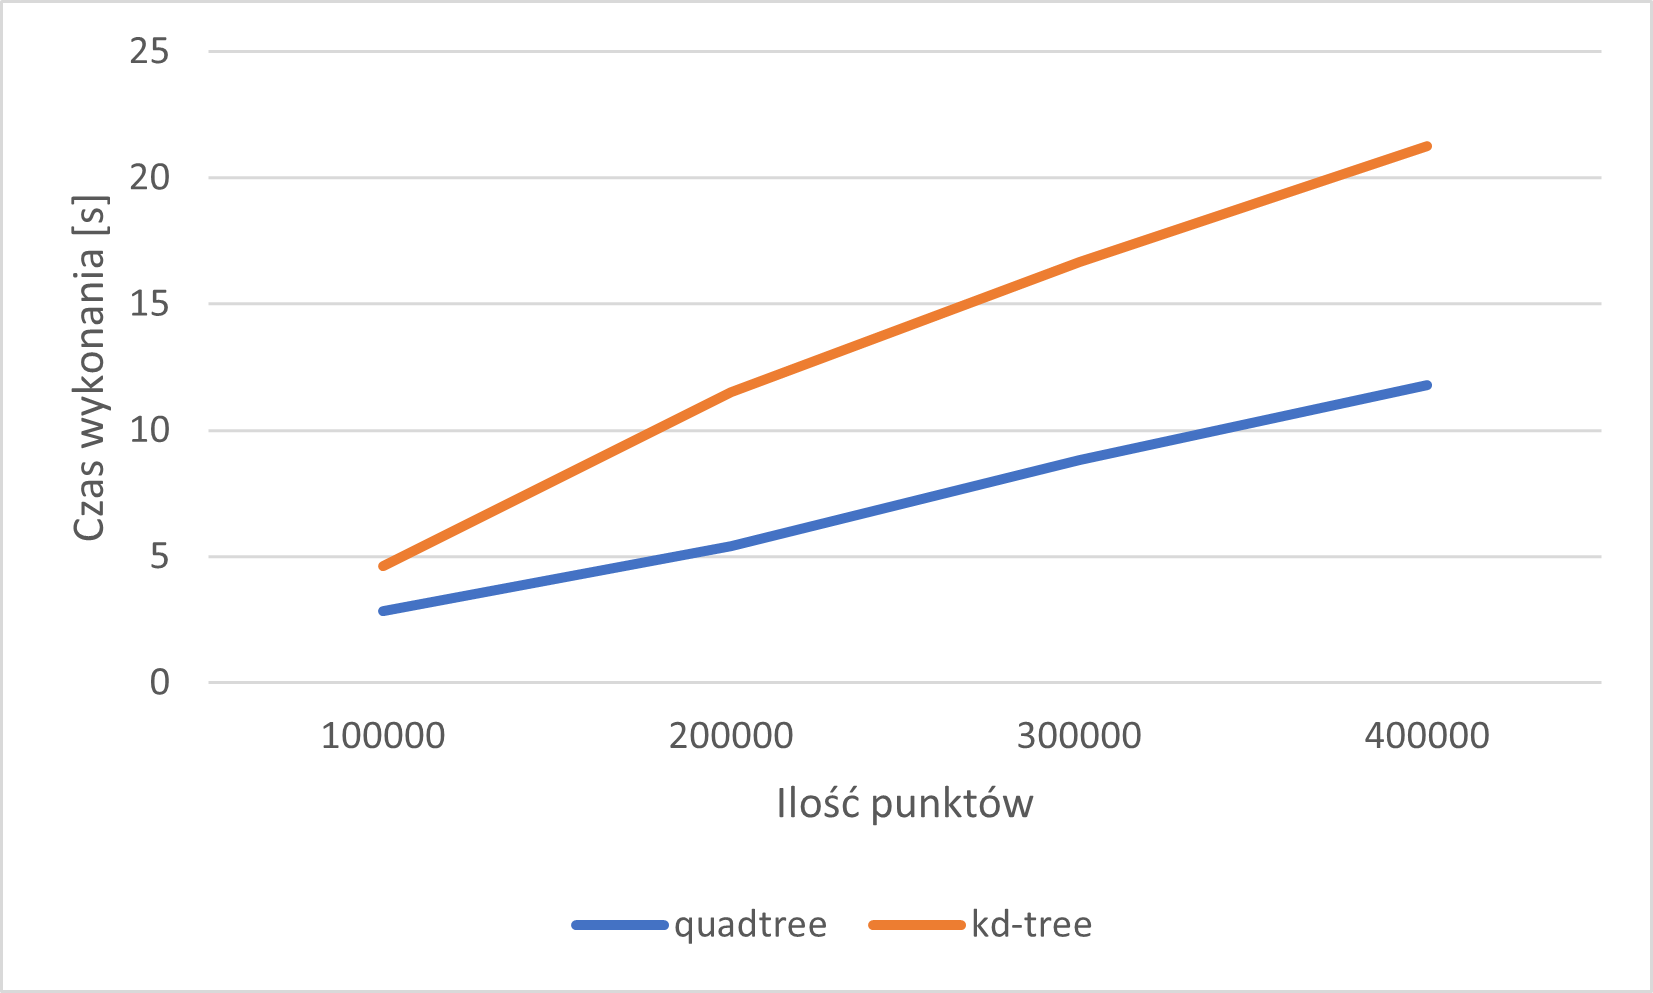
\includegraphics[width=\linewidth]{buildup_chart.png}
    \caption{Porównanie czasów budowania drzewa przez obie struktury}
    \label{fig:buildup_chart}
\end{figure}

\begin{figure}[H]
    \centering
    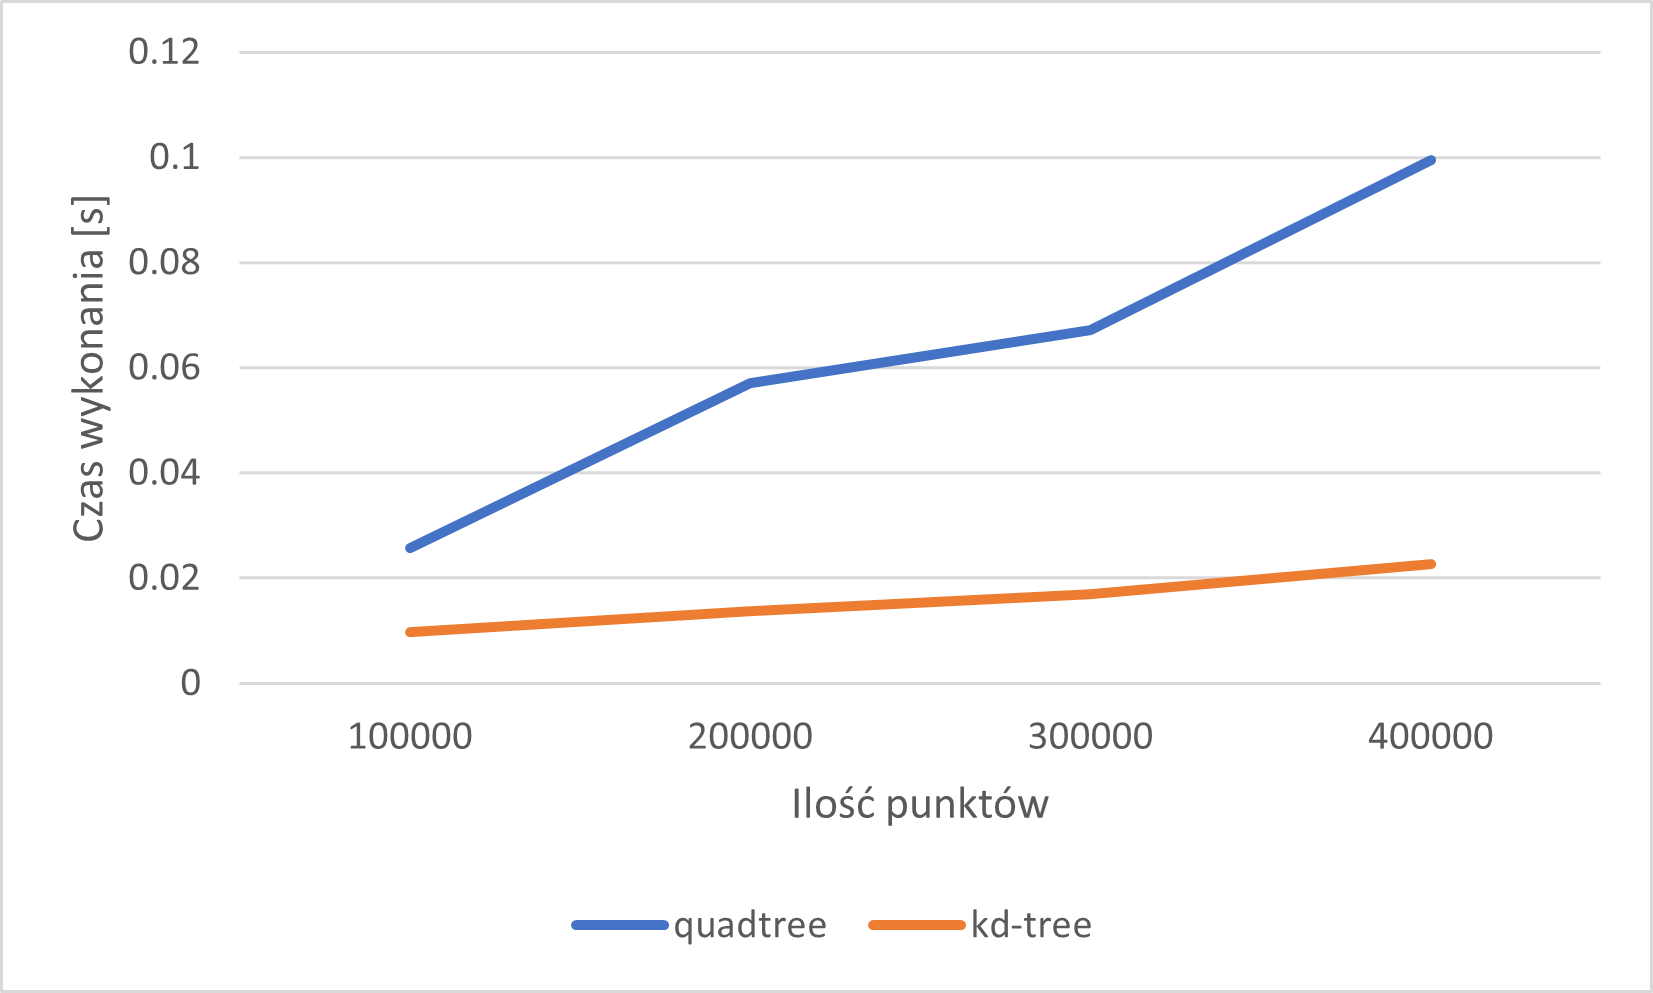
\includegraphics[width=\linewidth]{query_chart.png}
    \caption{Porównanie czasów wykonywania zapytań przez obie struktury}
    \label{fig:query_chart}
\end{figure}

\section{Bibliografia}

\begin{enumerate}
    \item dr inż. Barbara Głut \textit{Wykład -- wyszukiwanie geometryczne}
    \item Robert Bembenik \textit{Metody eksploracji danych z systemów informacji przestrzennej}, październik 2006
    \item mgr inż. Krzysztof Podsiadło \textit{narzędzie wizualizacyjne}
\end{enumerate}

\end{document}
